\documentclass[10pt]{article}
\usepackage[utf8]{inputenc}
\usepackage{amsmath}
\usepackage{amssymb}
\usepackage{enumitem}
\usepackage{ctex}
\usepackage{listings}
\usepackage{xcolor}
\usepackage[a4paper, margin=1in]{geometry}
\usepackage{hyperref}
\usepackage{graphicx}


\lstset{
    basicstyle=\ttfamily\small, % 设置代码字体和大小
    keywordstyle=\bfseries\color{blue}, % 设置关键字样式
    stringstyle=\color{red}, % 设置字符串样式
    commentstyle=\color{green}, % 设置注释样式
    numbers=left, % 显示行号
    numberstyle=\tiny\color{gray}, % 行号样式
    frame=single, % 添加边框
    breaklines=true, % 自动换行
    backgroundcolor=\color{gray!10} % 设置背景色
}

\title{项目报告}
% \author{Your Name}
% \date{\today}

\begin{document}

% \maketitle

    \tableofcontents
    \newpage


    \section{引言}

    \subsection{项目背景}

    随着社会的快速发展和人们生活水平的提高,交通出行需求日益增加。旅客在选择交通工具时,不同的出行目的和需求导致了对交通工具的多样化要求。例如,商务旅客希望在旅途中花费最少的时间,而旅游者则希望节省旅费,老年旅客则更关注中转次数的最少。为了满足不同旅客的需求,提供一个全国城市间的交通咨询程序显得尤为重要。

    \subsection{项目目标}
    本项目旨在开发一个全国交通咨询模拟系统,能够为旅客提供两种或三种最优决策的交通咨询服务。通过该系统,用户可以方便地查询从起始站到终点站的最快到达时间、最省钱的路线以及中转次数最少的方案,从而帮助旅客做出最佳的出行决策。

    \subsection{项目意义}
    本项目的实施将有助于提高旅客出行的效率,减少旅客的出行成本,提高旅客出行的舒适度。同时,本项目还有助于提高我国城市间交通运输的效率,减少交通拥堵,提高交通运输的安全性。


    \section{需求分析}

    \subsection{功能需求}
    本系统应具备以下功能:

    \begin{itemize}
        \item 用户可以输入起始站和终点站,选择最优决策原则(最快到达、最省钱到达、最少中转次数到达)和交通工具(火车、飞机),系统将提供相应的最优决策方案。
        \item 系统能够根据用户的输入,提供从起始站到终点站的最快到达时间、最省钱的路线和中转次数最少的方案。
        \item 系统能够显示每个方案的详细信息,包括列车或飞机的班次、出发和到达时间、票价等。
        \item 系统能够根据用户的需求,提供城市信息的编辑功能,包括添加或删除城市信息。
        \item 系统能够根据用户的需求,提供列车时刻表和飞机航班的编辑功能,包括增设或删除列车时刻表和飞机航班信息。
    \end{itemize}

    \subsection{非功能需求}
    本系统应满足以下非功能需求:

    \begin{itemize}
        \item 系统应具有良好的用户界面,易于用户使用和理解。
        \item 系统应具有高效的查询性能,能够快速地返回查询结果。
        \item 系统应具有良好的数据安全性,保护用户的个人信息和查询记录。
        \item 系统应具有良好的可扩展性,能够根据需求进行功能扩展和升级。
        \item 系统应具有良好的可靠性,能够在各种环境下稳定运行。
    \end{itemize}


    \section{系统设计}

    \subsection{系统架构}
    本系统采用前后端分离的架构,前端使用React框架进行开发,后端使用Python和FastAPI框架进行开发。前端负责用户界面,通过API与后端进行数据交互,后端负责处理业务逻辑和数据存储。

    \subsection{模块设计}
    系统主要分为以下几个模块:
    \begin{itemize}
        \item 数据存储模块:负责系统数据的存储和管理,生成可视化路线图代码。
        \item 城市信息管理模块:提供城市信息的添加、删除、修改等功能。
        \item 交通工具管理模块:提供列车时刻表和飞机航班的编辑功能。
        \item 路线规划模块:根据用户输入的起始站、终点站和最优决策原则,提供相应的最优路线。
    \end{itemize}

    \subsection{数据存储设计}
    系统使用简易的json格式的文件存储数据,主要包括以下几个文件:
    \begin{itemize}
        \item 城市表:存储城市的基本信息。
        \item 路线表:存储各城市之间的交通路线信息。
    \end{itemize}


    \section{详细设计}

    \subsection{存储结构设计}

    \subsubsection{城市表}
    城市信息以json格式存储,每个城市包括以下字段:
    \begin{lstlisting}[language=Python]
[
    {
        "name": "上海"
    }
]
    \end{lstlisting}
    其中,name字段表示城市的名称。

    \subsubsection{路线表}
    路线信息以json格式存储,每个路线包括以下字段:
    \begin{lstlisting}[language=Python]
[
    {
    "type": "train",
    "name": "T169",
    "start": "上海",
    "end": "杭州",
    "price": 28,
    "start_time": "11:26",
    "end_time": "13:29",
    "run_id": "T169"
    }
]
    \end{lstlisting}
    其中:
    \begin{itemize}
        \item type字段表示交通工具类型(火车或飞机)。
        \item name字段表示交通工具的名称。
        \item start字段表示出发城市。
        \item end字段表示到达城市。
        \item price字段表示票价。
        \item start\_time字段表示出发时间。
        \item end\_time字段表示到达时间。
        \item run\_id字段表示班次。
    \end{itemize}

    \subsection{数据结构设计}

    系统会把在磁盘上以列表的形式存储的城市信息和路线信息读入内存,然后构建一个图数据结构,用于路线规划。图数据结构的节点表示城市,边表示城市之间的交通路线。
    本次课程设计沿用了实验设计的图数据结构,具体实现如下:

    \subsubsection{Node 接口:表示图的节点}
    \begin{itemize}[label=\textbullet]
        \item \textbf{抽象方法:}
        \begin{itemize}[label=\textbullet]
            \item \texttt{\_\_init\_\_(self, value: T = None)}: 初始化节点,持有一个值 \texttt{value}。
            \item \texttt{add\_edge(self, node: \"Node\", value: U) -> \"Edge\"}: 从当前节点添加一条指向 \texttt{node} 的有向边,边的值为 \texttt{value}。
            \item \texttt{destroy(self)}: 从图中删除当前节点,以及所有关联的边。
        \end{itemize}
        \item \textbf{属性:}
        \begin{itemize}[label=\textbullet]
            \item \texttt{value}: 节点存储的值。
            \item \texttt{edges}: 以当前节点为起点的出边的迭代器。
            \item \texttt{rev\_edges}: 以当前节点为终点的入边的迭代器。
        \end{itemize}
    \end{itemize}

    \subsubsection{Edge 接口:表示图的边}
    \begin{itemize}[label=\textbullet]
        \item \textbf{抽象方法:}
        \begin{itemize}[label=\textbullet]
            \item \texttt{\_\_init\_\_(self, from\_node: Node, to\_node: Node, value: U = None)}: 初始化边,指定起点 \texttt{from\_node}、终点 \texttt{to\_node} 和边的值 \texttt{value}。
            \item \texttt{destroy(self)}: 从图中删除当前边。
        \end{itemize}
        \item \textbf{属性:}
        \begin{itemize}[label=\textbullet]
            \item \texttt{value}: 边存储的值。
            \item \texttt{from\_node}: 边的起点节点。
            \item \texttt{to\_node}: 边的终点节点。
        \end{itemize}
    \end{itemize}

    \subsubsection{Graph 接口:表示图结构,包含节点和边}
    \begin{itemize}[label=\textbullet]
        \item \textbf{抽象方法:}
        \begin{itemize}[label=\textbullet]
            \item \texttt{\_\_init\_\_(self)}: 初始化图对象。
            \item \texttt{add\_node(self, value: T) -> Node}: 向图中添加一个值为 \texttt{value} 的节点。
            \item \texttt{get\_nodes\_func(self, func: Callable[[T], bool]) -> Iterator[Node]}: 根据条件函数 \texttt{func} 查找节点。
            \item \texttt{get\_edges\_func(self, func: Callable[[U], bool]) -> Iterator[Edge]}: 根据条件函数 \texttt{func} 查找边。
        \end{itemize}
        \item \textbf{方法:}
        \begin{itemize}[label=\textbullet]
            \item \texttt{get\_nodes(self, value: T) -> Iterator[Node]}: 根据值 \texttt{value} 查找节点,使用等于运算符。
            \item \texttt{get\_edges(self, value: U) -> Iterator[Edge]}: 根据值 \texttt{value} 查找边,使用等于运算符。
        \end{itemize}
    \end{itemize}

    这些接口定义了图、节点和边的基本结构和操作,为具体的图实现提供了规范。

    \subsection{算法设计}
    根据需求,系统需要实现以下几种算法:
    \begin{itemize}
        \item 最短路径算法:根据用户输入的最优决策原则,计算从起始站到终点站的最短路径。
        \item 最省钱算法:根据用户输入的最优决策原则,计算从起始站到终点站的最省钱路径。
        \item 最少中转次数算法:根据用户输入的最优决策原则,计算从起始站到终点站的最少中转次数路径。
    \end{itemize}

    \subsubsection{算法设计难点}
    交通工具的出发时间是固定的,这使得路径规划变得复杂。我们需要在考虑交通工具运行时间的前提下,选择总时间最小的路径。具体难点包括:

    \begin{itemize}
        \item \textbf{时间约束}: 每个交通工具的出发时间是固定的,必须在合适的时间到达中转站以赶上下一班交通工具。
        \item \textbf{等待时间}: 在中转站的等待时间需要纳入总时间计算中,选择合适的中转站和中转时间至关重要。
        \item \textbf{多目标优化}: 需要在最短时间和最少费用之间进行权衡,有时需要在多个最优解之间进行选择。
        \item \textbf{数据规模}: 交通网络可能非常庞大,涉及多个城市和交通工具,计算复杂度较高。
    \end{itemize}

    \subsubsection{最省钱路径}

    最省钱路径的计算使用了 Dijkstra 算法。Dijkstra 算法是一种经典的单源最短路径算法,适用于边权非负的图。为了计算从起始站到终点站的最省钱路径,我们将票价作为边的权重,使用 Dijkstra 算法进行路径规划。

    \paragraph{算法步骤}
    \begin{enumerate}
        \item 初始化:将起始站的费用设为0,其他所有节点的费用设为无穷大。将所有节点标记为未访问。
        \item 选择当前费用最小的未访问节点作为当前节点,标记为已访问。
        \item 更新当前节点的邻接节点的费用。如果通过当前节点到达某个邻接节点的费用小于当前记录的费用,则更新该邻接节点的费用。
        \item 重复步骤2和3,直到所有节点都被访问过或当前节点的费用为无穷大。
        \item 从终点站回溯,构建最省钱路径。
    \end{enumerate}

    \paragraph{伪代码}
    \begin{lstlisting}[language=Python]
def dijkstra(graph, start, end):
    import heapq
    pq = []
    heapq.heappush(pq, (0, start))
    costs = {node: float('inf') for node in graph.nodes}
    costs[start] = 0
    parents = {node: None for node in graph.nodes}

    while pq:
        current_cost, current_node = heapq.heappop(pq)

        if current_node == end:
            break

        for neighbor, weight in graph.edges[current_node]:
            new_cost = current_cost + weight
            if new_cost < costs[neighbor]:
                costs[neighbor] = new_cost
                parents[neighbor] = current_node
                heapq.heappush(pq, (new_cost, neighbor))

    path = []
    node = end
    while node:
        path.append(node)
        node = parents[node]
    path.reverse()

    return path, costs[end]
    \end{lstlisting}

    \paragraph{复杂度分析}
    Dijkstra 算法的时间复杂度为 $O((|V| + |E|) \log |V|)$,其中 $|V|$ 是节点数,$|E|$ 是边数。由于我们使用了优先队列(堆)来选择当前费用最小的节点,因此算法在大多数情况下都能高效运行。

    \subsubsection{最少中转次数路径}

    最少中转次数路径的计算可以基于 Dijkstra 算法进行修改。我们将边的权重定义为中转次数:如果两个节点之间的交通工具相同,则权重为0;否则,权重为1。这样,Dijkstra 算法计算出的最短路径即为最少中转次数路径。

    \paragraph{算法步骤}
    \begin{enumerate}
        \item 初始化:将起始站的中转次数设为0,其他所有节点的中转次数设为无穷大。将所有节点标记为未访问。
        \item 选择当前中转次数最小的未访问节点作为当前节点,标记为已访问。
        \item 更新当前节点的邻接节点的中转次数。具体规则是:如果两个节点之间的交通工具相同且班次相同,则中转次数不变;否则,中转次数加1。如果通过当前节点到达某个邻接节点的中转次数小于当前记录的中转次数,则更新该邻接节点的中转次数。
        \item 重复步骤2和3,直到所有节点都被访问过或当前节点的中转次数为无穷大。
    \end{enumerate}

    \paragraph{伪代码} 和上文中的伪代码类似,在此处不再赘述。

    \paragraph{复杂度分析} 同样,时间复杂度为 $O((|V| + |E|) \log |V|)$。

    \subsubsection{最快到达路径}

    最快到达路径的计算同样基于 Dijkstra 算法,但是需要设置全局统一的起始时间,基于此时间计算第一条边的花费,然后再基于当前边,计算下一条边的花费,最后最小花费即为最快到达的路径。

    \paragraph{算法步骤}
    \begin{enumerate}
        \item 初始化:将起始站的时间设为0,其他所有节点的时间设为无穷大。将所有节点标记为未访问。
        \item 选择当前时间最小的未访问节点作为当前节点,标记为已访问。
        \item 更新当前节点的邻接节点的时间。具体规则是:计算从当前节点到达邻接节点的时间,如果通过当前节点到达某个邻接节点的时间小于当前记录的时间,则更新该邻接节点的时间。
        \item 重复步骤2和3,直到所有节点都被访问过或当前节点的时间为无穷大。
    \end{enumerate}

    \paragraph{伪代码} 和上文类似,此处不再赘述。

    \paragraph{复杂度分析} 同样,时间复杂度为 $O((|V| + |E|) \log |V|)$。

    \subsubsection{时间段的合理计算}
    为了准确计算最快到达路径,需要定义合理的时间计算规则,特别是处理过夜的情况。以下是时间计算的具体规则:

    \begin{itemize}
        \item \textbf{时间格式}: 所有时间均采用24小时制,格式为HH:MM。
        \item \textbf{时间差计算}: 计算两个时间点之间的差值时,需考虑是否跨越午夜。例如,从23:00到01:00的时间差为2小时。
        \item \textbf{等待时间}: 在中转站的等待时间需纳入总时间计算中。等待时间的计算规则与时间差计算相同,需考虑是否跨越午夜。
        \item \textbf{出发时间约束}: 每个交通工具的出发时间是固定的,必须在合适的时间到达中转站以赶上下一班交通工具。如果到达时间晚于下一班交通工具的出发时间,则需等待至下一班交通工具的出发时间。
    \end{itemize}

    通过以上规则,可以确保在计算最快到达路径时,能够准确处理时间差和过夜问题,从而得到合理的结果。

    \subsection{接口设计}
    系统采用REST风格的API设计,主要包含以下几个模块的接口:

    \subsubsection{城市管理接口}
    \begin{itemize}
        \item \textbf{获取城市列表}
        \begin{itemize}
            \item 请求方法:GET
            \item 路径:/api/cities
            \item 响应:返回所有城市信息的列表
        \end{itemize}
        \item \textbf{添加城市}
        \begin{itemize}
            \item 请求方法:POST
            \item 路径:/api/cities
            \item 请求体:城市信息(名称)
            \item 响应:添加成功的状态
        \end{itemize}
        \item \textbf{删除城市}
        \begin{itemize}
            \item 请求方法:POST
            \item 路径:/api/cities/delete
            \item 响应:删除成功的状态
        \end{itemize}
    \end{itemize}

    \subsubsection{交通路线管理接口}
    \begin{itemize}
        \item \textbf{获取交通路线}
        \begin{itemize}
            \item 请求方法:GET
            \item 路径:/api/transports
            \item 响应:返回所有交通路线信息的列表
        \end{itemize}
        \item \textbf{添加交通路线}
        \begin{itemize}
            \item 请求方法:POST
            \item 路径:/api/transports
            \item 请求体:路线信息(类型、班次、起始站、终点站、价格、时间等)
            \item 响应:添加成功的状态
        \end{itemize}
        \item \textbf{删除交通路线}
        \begin{itemize}
            \item 请求方法:POST
            \item 路径:/api/transports/delete
            \item 响应:删除成功的状态
        \end{itemize}
    \end{itemize}

    \subsubsection{路线规划接口}
    \begin{itemize}
        \item \textbf{路线规划查询}
        \begin{itemize}
            \item 请求方法:GET
            \item 路径:/api/routes/plan
            \item 查询参数:
            \begin{itemize}
                \item start:起始站
                \item end:终点站
                \item strategy:规划策略(最快/最省钱/最少中转)
                \item start\_time:出发时间(当策略为最快时必需)
            \end{itemize}
            \item 响应:返回规划结果,包含路线详情、总时间和总价格、以及路线地图
        \end{itemize}
    \end{itemize}


    \section{实现}

    \subsection{开发环境}
    本项目的开发环境如下:
    \begin{itemize}
        \item 集成开发环境:PyCharm 2024.2.5
        \item 编程语言:Python 3.12
        \item 后端框架:FastAPI 0.115.6
        \item 前端框架:React 18
        \item 操作系统:Windows 11
        \item 版本控制:Git 2.45.0
    \end{itemize}

    \subsection{图的邻接表实现}

    \subsubsection{整体设计思路}
    该实现采用邻接表的方式存储图结构,主要包含三个核心类:
    \begin{itemize}[label=\textbullet]
        \item \texttt{AdjacencyListGraph}: 图的主体类。
        \item \texttt{AdjacencyListNode}: 图中的节点类。
        \item \texttt{AdjacencyListEdge}: 图中的边类。
    \end{itemize}

    \subsubsection{数据存储结构}

    \paragraph{图的存储}
    \begin{itemize}[label=\textbullet]
        \item 图类(\texttt{AdjacencyListGraph})内部维护了一个节点列表 \texttt{\_nodes}。
        \item 所有的节点都存储在这个列表中,便于整体管理和遍历。
    \end{itemize}

    \paragraph{节点的存储}
    \begin{itemize}[label=\textbullet]
        \item 每个节点(\texttt{AdjacencyListNode})包含:
        \begin{itemize}[label=\textbullet]
            \item 节点值(\texttt{\_value})。
            \item 一个边集合(\texttt{\_edge})存储从该节点出发的所有边。
            \item 对所属图的引用(\texttt{\_graph})。
        \end{itemize}
    \end{itemize}

    \paragraph{边的存储}
    \begin{itemize}[label=\textbullet]
        \item 每条边(\texttt{AdjacencyListEdge})记录:
        \begin{itemize}[label=\textbullet]
            \item 起始节点(\texttt{\_from\_node})。
            \item 目标节点(\texttt{\_to\_node})。
            \item 边的权值(\texttt{\_value})。
            \item 对所属图的引用(\texttt{\_graph})。
        \end{itemize}
    \end{itemize}

    \subsubsection{关键实现特点}

    \paragraph{邻接表特性}
    \begin{itemize}[label=\textbullet]
        \item 每个节点维护一个从该节点出发的边的集合。
        \item 这种存储方式特别适合稀疏图,因为只存储实际存在的边。
        \item 空间复杂度为 $O(|V| + |E|)$,其中 $|V|$ 是节点数,$|E|$ 是边数。
    \end{itemize}

    \paragraph{双向查询支持}
    \begin{itemize}[label=\textbullet]
        \item 可以快速获取从某个节点出发的所有边(通过节点的 \texttt{\_edge} 集合)。
        \item 也支持查询指向某个节点的所有边(通过图的边遍历实现)。
    \end{itemize}

    \paragraph{节点和边的关联}
    \begin{itemize}[label=\textbullet]
        \item 每个节点和边都保持对图的引用,确保它们能访问图的整体信息。
        \item 边对象同时保持对其起始节点和终止节点的引用,便于导航。
    \end{itemize}

    \subsection{最省钱路径规划实现}
    \begin{lstlisting}[language=Python]
    @staticmethod
    def cheapest(tm: TransportMap, start: str, end: str) -> list[Transport]:
        '''Dijkstra算法,不需要考虑时间,只考虑价格'''
        start_node = tm.data.get_node(start)
        end_node = tm.data.get_node(end)
        pri_queue = queue.PriorityQueue()
        pri_queue.put((0, start_node, [start_node]))
        visited = set()
        while not pri_queue.empty():
            distance, node, path = pri_queue.get()
            if node in visited:
                continue
            visited.add(node)
            if node == end_node:
                return [edge.value for edge in path if isinstance(edge.value, Transport)]
            for edge in node.edges:
                pri_queue.put((distance + edge.value.price, edge.to_node, path + [edge]))
        return []
    \end{lstlisting}

    \subsubsection{最少中转次数路径规划实现}

    \begin{lstlisting}[language=Python]
    @staticmethod
    def transfer_count_least_v2(tm: TransportMap, start: str, end: str) -> list[Transport]:
        '''Dijkstra算法'''
        start_node = tm.data.get_node(start)
        end_node = tm.data.get_node(end)
        pri_queue = queue.PriorityQueue()
        pri_queue.put((0, start_node, []))
        visited = set()
        while not pri_queue.empty():
            distance, node, path = pri_queue.get()
            if node in visited:
                continue
            visited.add(node)
            if node == end_node:
                return [edge.value for edge in path if isinstance(edge.value, Transport)]
            for edge in node.edges:
                if path:
                    pri_queue.put((distance + (edge.value.run_id != path[-1].value.run_id), edge.to_node, path + [edge]))
                else:
                    pri_queue.put((distance, edge.to_node, path + [edge]))
        return []
    \end{lstlisting}

    \subsubsection{最快时间路径规划实现}
    \begin{lstlisting}[language=Python]
    @staticmethod
    def fastest_v3(tm: TransportMap, start: str, end: str, start_time: int | str | TimeSegment) -> list[Transport]:
        '''基于Dijkstra思想,找到耗时最短的路径'''
        if not isinstance(start_time, TimeSegment):
            start_time = TimeSegment(start_time, start_time)
        start_node = tm.data.get_node(start)
        end_node = tm.data.get_node(end)
        pri_queue: queue.PriorityQueue[tuple[TimeSegment, Node, list[Edge[Transport]]]] = queue.PriorityQueue()
        pri_queue.put((start_time, start_node, []))
        visited = set()
        while not pri_queue.empty():
            current_time, node, path = pri_queue.get()
            if node in visited:
                continue
            visited.add(node)
            if node == end_node:
                return [edge.value for edge in path if isinstance(edge.value, Transport)]
            # 给 edge 按照 node 分组
            edges: dict[Node, list[Edge[Transport]]] = defaultdict(list[Edge[Transport]])
            to_nodes = set()
            for edge in node.edges:
                edges[edge.to_node].append(edge)
                to_nodes.add(edge.to_node)
            # 优先选择加上等待时间,到达目的地最早的交通工具
            for to_node in to_nodes:
                def calc_real_cost_time(edge: Edge[Transport]) -> TimeSegment:
                    '''计算实际的时间'''
                    return current_time + TimeSegment(edge.value.start_time, edge.value.end_time)

                edge = min(edges[to_node], key=lambda e: calc_real_cost_time(e))
                pri_queue.put(
                    (calc_real_cost_time(edge), edge.to_node, path + [edge]))
        return []
    \end{lstlisting}


    \section{测试}

    \subsection{测试用例}

    \subsubsection{全量数据}

    实现一个可用的路径规划系统需要大量数据,所以从网络采集了大量铁路交通和航班的数据,并使用 Python 进行数据处理,生成一个可用的交通工具列表。
    目前一共收集了15个城市和4130条交通工具的数据:
    \begin{lstlisting}[language=Python]
[
  {
    "name": "上海"
  },
  {
    "name": "北京"
  },
  {
...
    \end{lstlisting}

    \begin{lstlisting}[language=Python]
[
  {
    "type": "train",
    "name": "T169",
    "start": "上海",
    "end": "杭州",
    "price": 28,
    "start_time": "11:26",
    "end_time": "13:29",
    "run_id": "T169"
  },
  {
    "type": "train",
    "name": "T169",
    "start": "杭州",
    "end": "广州",
    "price": 161,
    "start_time": "1
...
    \end{lstlisting}
    由于数据量过大,无法直接展示,这里只展示一部分数据。更多数据请访问项目仓库\ref{项目仓库}中的数据文件\ref{city_data}和\ref{transport_data}。
    \subsubsection{特挑数据}
    为了更好的展现算法的效果,我选择了部分数据组成了几个有代表性的数据集。详情请查看\ref{项目仓库}

    \subsection{测试结果}
    项目提供了一个功能完善的前端页面,所以测试相关的操作都在前端完成


    目前主要分为四个模块,分别是路径规划、地点查询、路线查询和路线图。同时,最左边有一个下拉输入框,允许用户选择不同的数据集(例如全量数据)来进行路径规划。

    \paragraph{路径规划} 如图\ref{fig:screenshot001}所示:
    \begin{enumerate}
        \item 城市选择:用户需要选择起始城市和目标城市。这可以通过下拉菜单来完成,菜单中列出了可选的城市列表。
        \item 规划策略:用户可以选择三种不同的规划策略:
        \begin{itemize}
            \item 最快:选择此选项将优先考虑时间最短的路线。
            \item 最省钱:选择此选项将优先考虑成本最低的路线。
            \item 最少中转:选择此选项将优先考虑中转次数最少的路线。
        \end{itemize}
        \item 开始时间:用户可以设置出发的具体时间。在当前示例中,已经设置了出发时间为08:00。
        \item 开始规划:点击这个按钮后,系统将根据用户的选择生成相应的路径规划方案。
    \end{enumerate}
    \begin{figure}
        \centering
        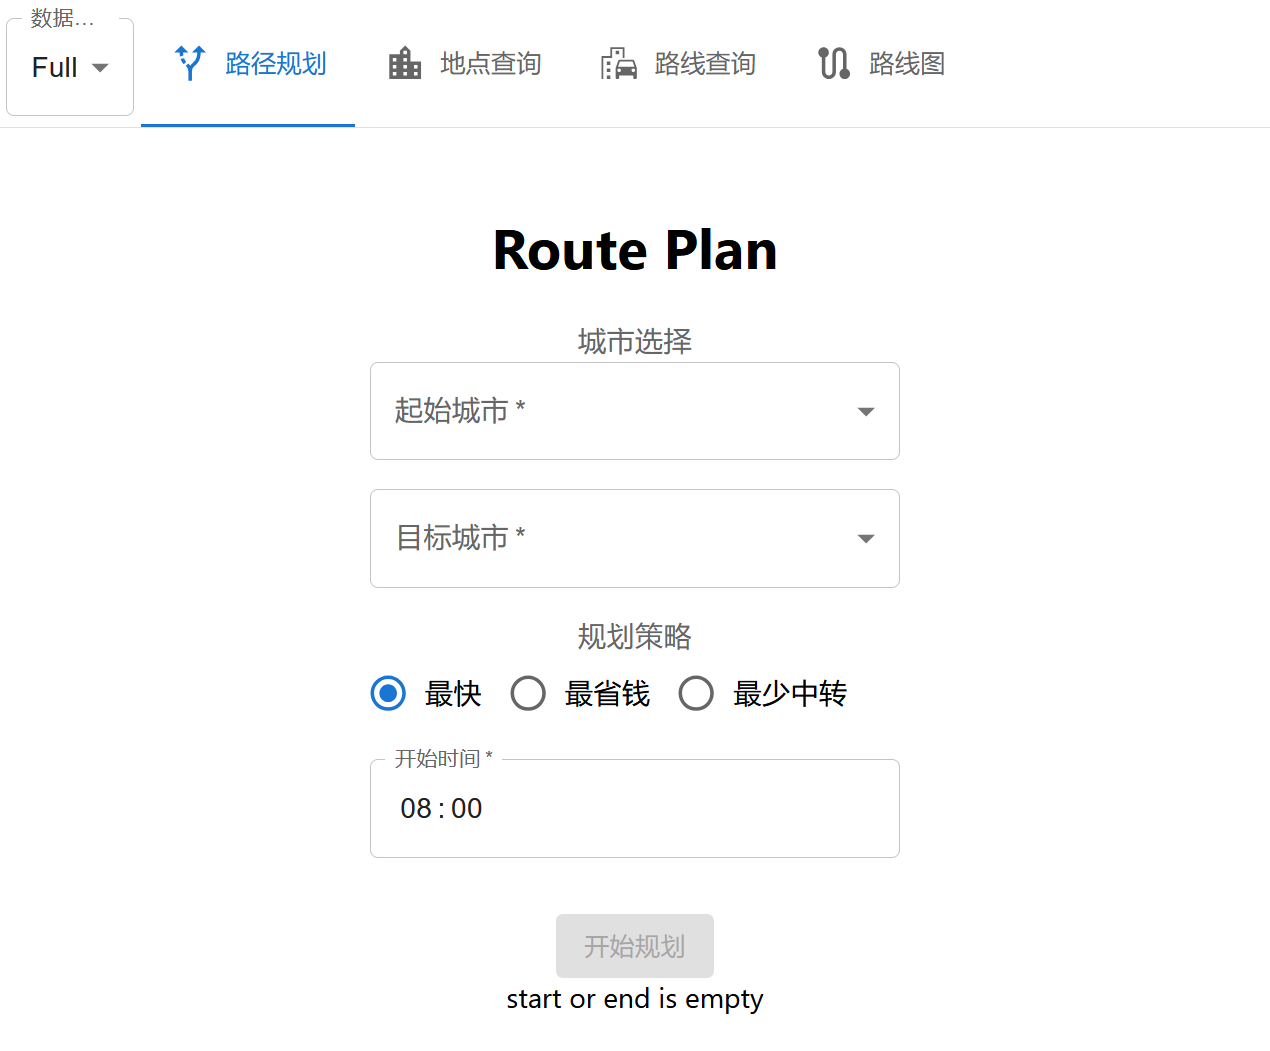
\includegraphics[width=\linewidth]{img/screenshot001}
        \caption[]{路径规划}
        \label{fig:screenshot001}
    \end{figure}

    \paragraph{地点查询} 图如\ref{fig:screenshot004}所示:
    \begin{enumerate}
        \item 城市查询:这是一个列表,用户可以在这里看到所有的城市。
        \item 删除城市:用户可以城市列表中的城市进行删除(存在交通方式的城市不能删除)。
        \item 添加城市:用户可以添加表单添加一个新的城市。
    \end{enumerate}
    \begin{figure}
        \centering
        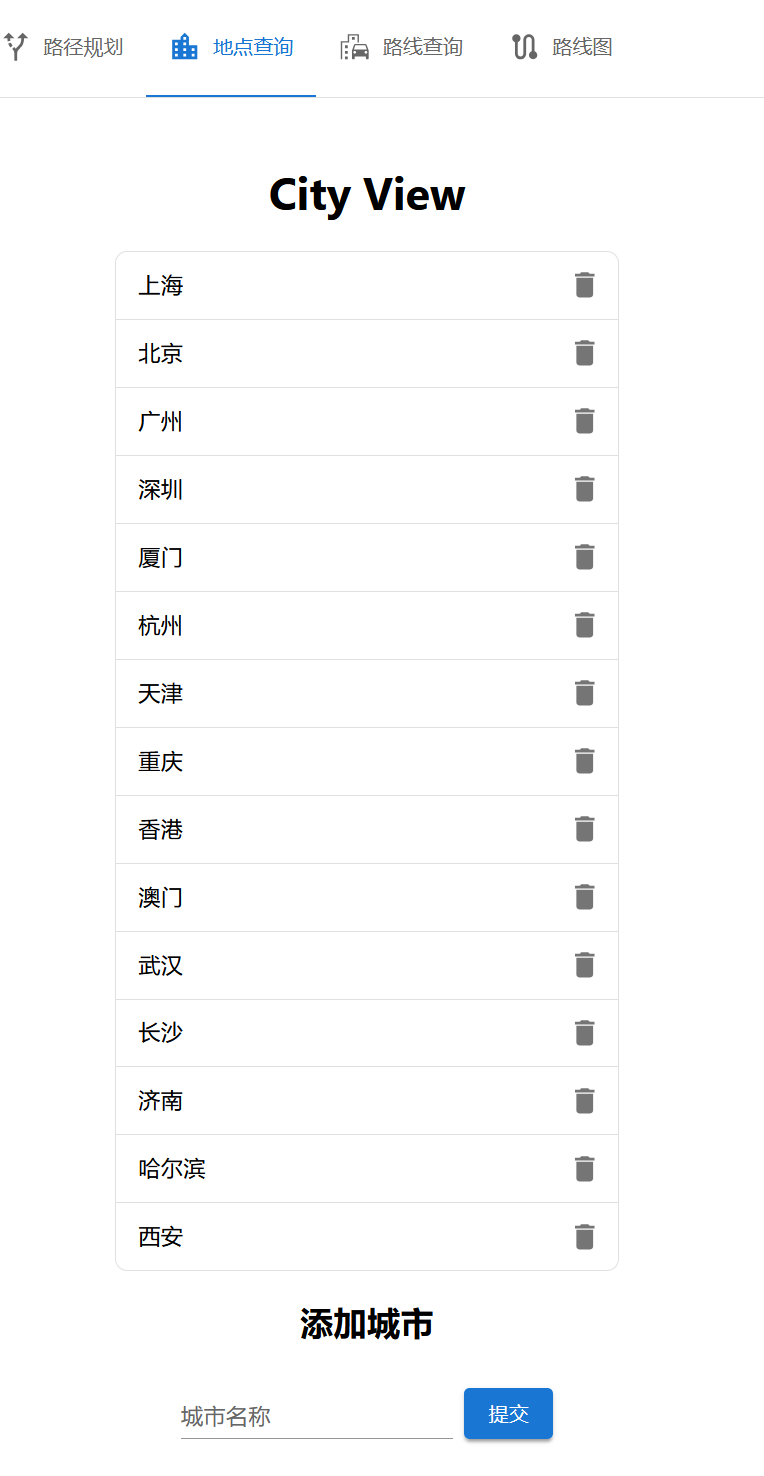
\includegraphics[width=0.5\linewidth]{img/screenshot004}
        \caption{地点查询}
        \label{fig:screenshot004}
    \end{figure}

    \paragraph{路线查询} 如图\ref{fig:screenshot006}所示:
    \begin{enumerate}
        \item 路线查询:这是一个列表,用户可以在这里看到所有的路线。
        \item 删除路线:用户可以路线列表中的路线进行删除。
        \item 路线筛选:用户可以通过交通方式、出发和目的地筛选出符合条件的路线。
        \item 添加路线:用户可以填写表单添加一个新的路线。
    \end{enumerate}
    \begin{figure}
        \centering
        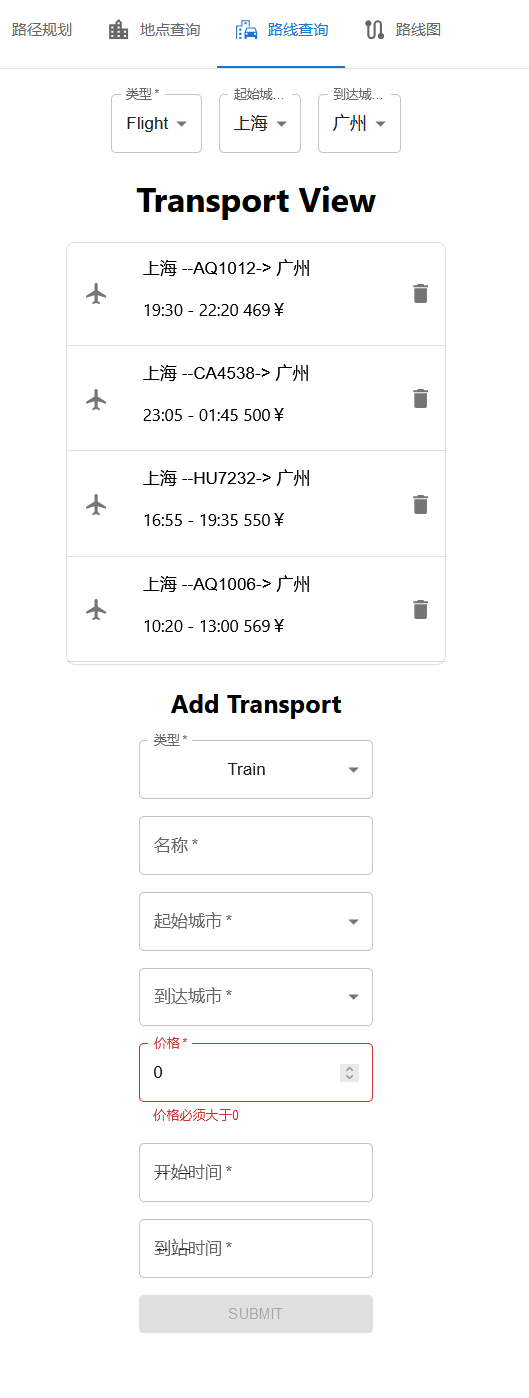
\includegraphics[width=0.5\linewidth]{img/screenshot006}
        \caption[]{路线查询}
        \label{fig:screenshot006}
    \end{figure}

    \paragraph{路线图} 如图\ref{fig:screenshot007}所示:
    \begin{enumerate}
        \item 显示路线:将系统内的所有路线以可视化的图形展示出来(仅小数据时可用)。
    \end{enumerate}
    \begin{figure}
        \centering
        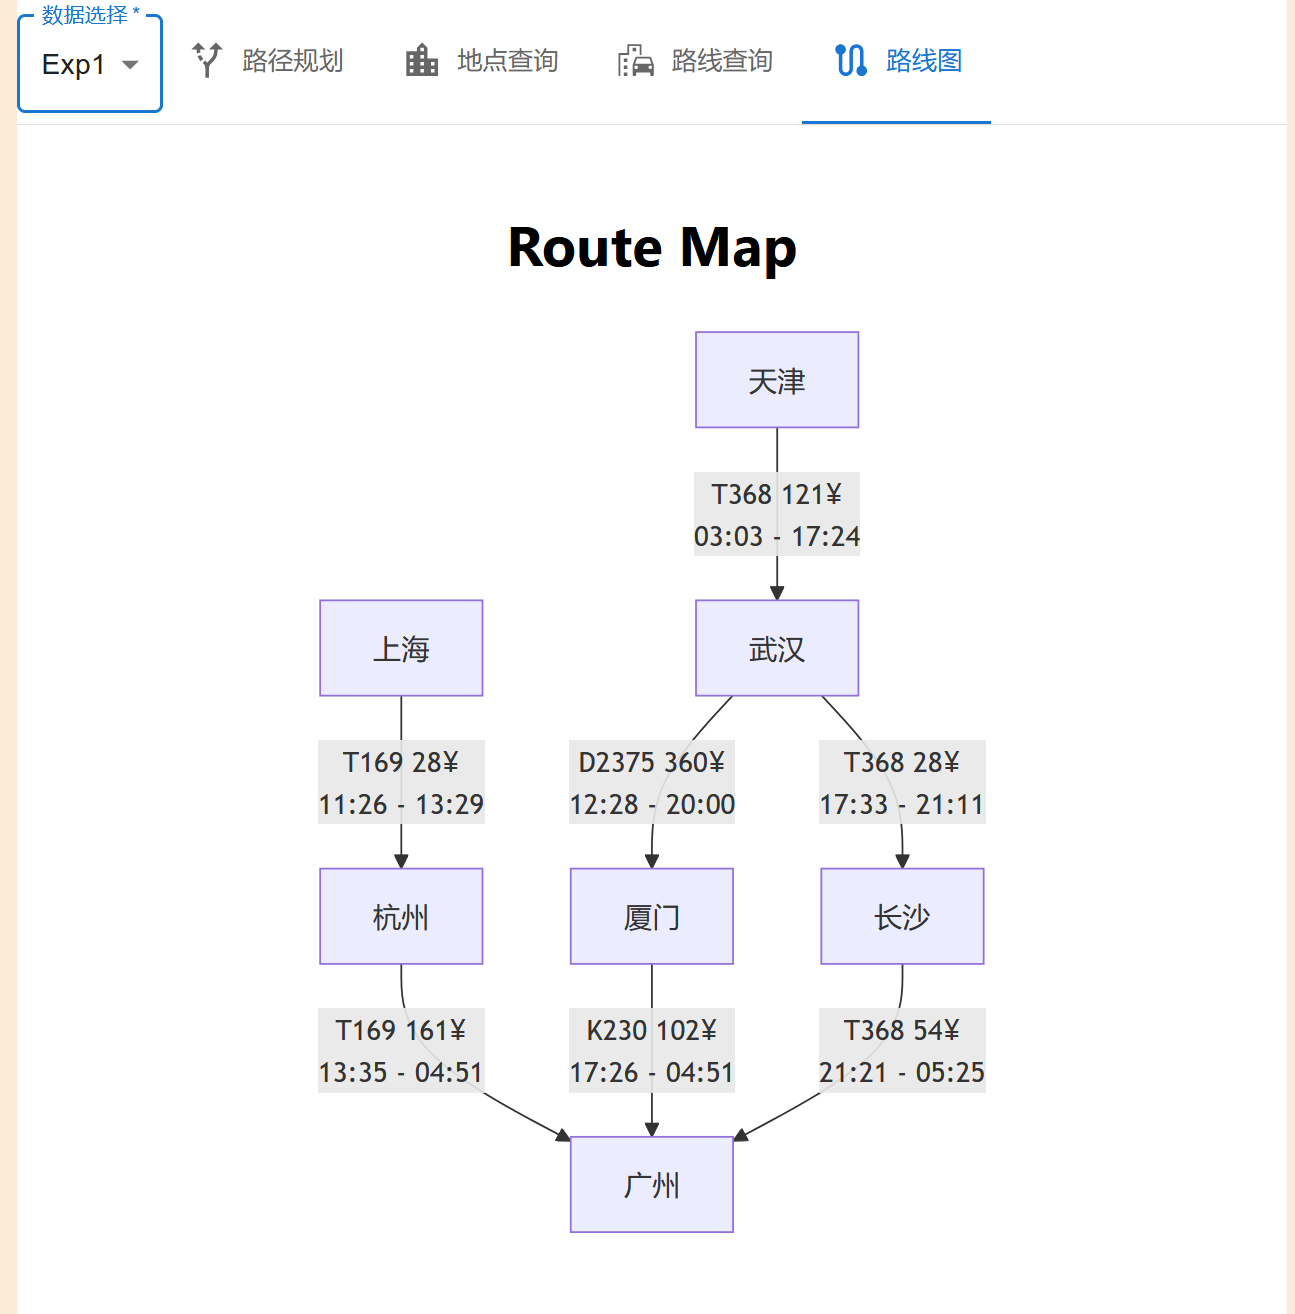
\includegraphics[width=0.7\linewidth]{img/screenshot007}
        \caption{路线图}
        \label{fig:screenshot007}
    \end{figure}

    \subsubsection{最省钱路径规划}
    \begin{enumerate}
        \item 从上海到北京的最省钱路径规划结果,如图\ref{fig:screenshot002}所示。
    \end{enumerate}

    \subsubsection{最少中转路径规划}
    \begin{enumerate}
        \item 从上海到北京的最少中转路径规划结果,图如\ref{fig:screenshot003}所示。
    \end{enumerate}

    \begin{figure}[htbp]
        \centering
        \begin{minipage}[b]{0.45\linewidth}
            \centering
            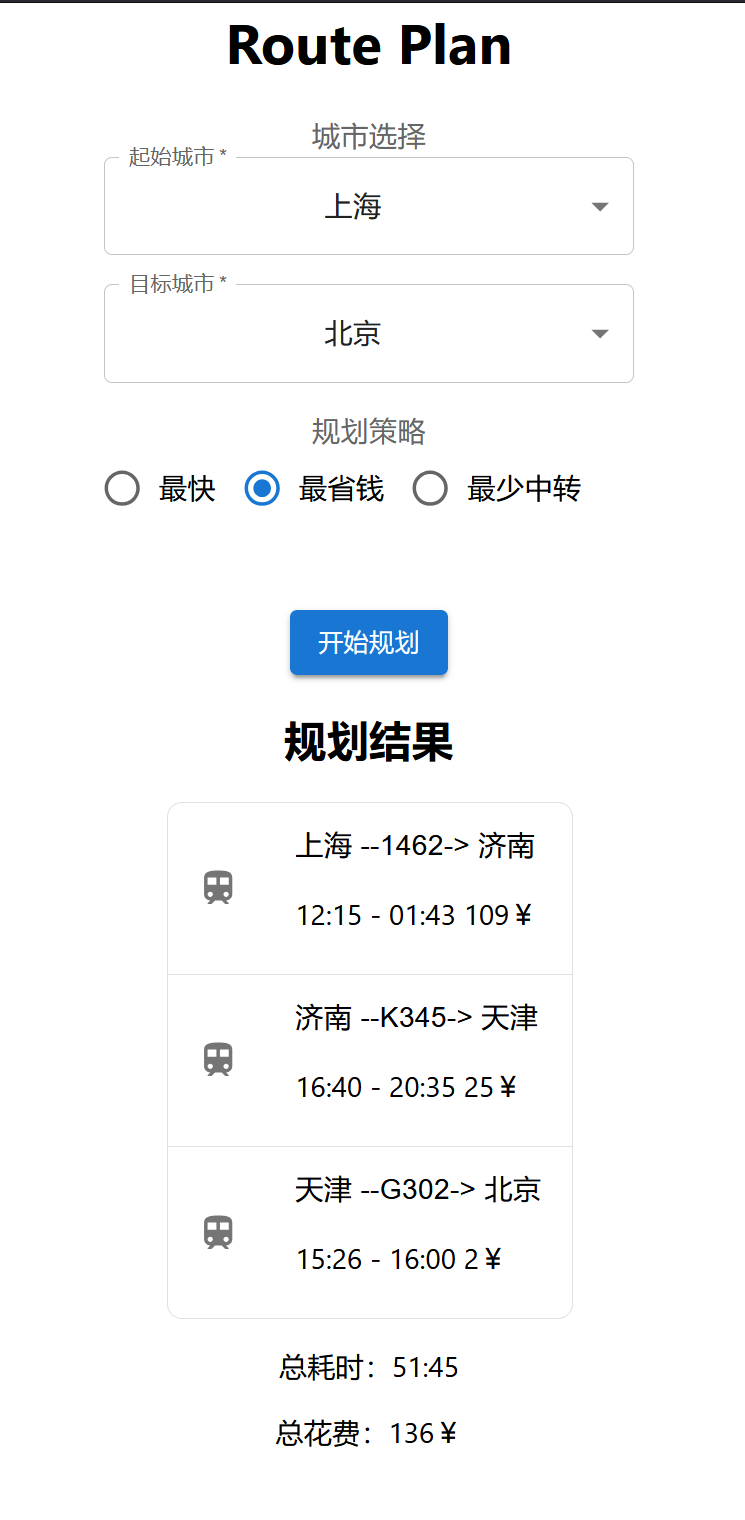
\includegraphics[width=\linewidth]{img/screenshot002}
            \caption{最省钱路径规划结果}
            \label{fig:screenshot002}
        \end{minipage}
        \hspace{0.05\linewidth}
        \begin{minipage}[b]{0.45\linewidth}
            \centering
            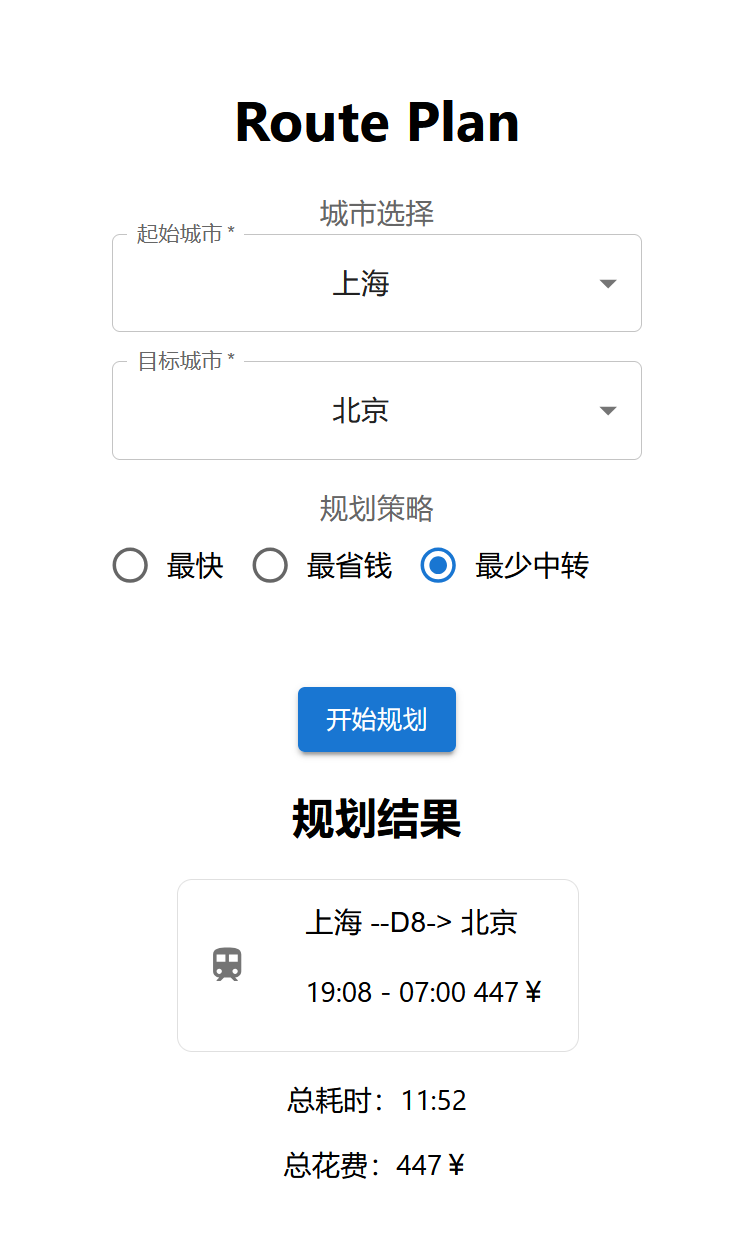
\includegraphics[width=\linewidth]{img/screenshot003}
            \caption{最少中转路径规划结果}
            \label{fig:screenshot003}
        \end{minipage}
    \end{figure}

    \subsubsection{最快路径规划算法}

    \paragraph{exp1-1}
    在当前的情况下,如图\ref{fig:screenshot008}所示,途径长沙。

    因为从武汉起步,如果途径厦门,由于到达之后下一程需要隔日才能发车,所以优先选择了途径长沙。
    \begin{figure}
        \centering
        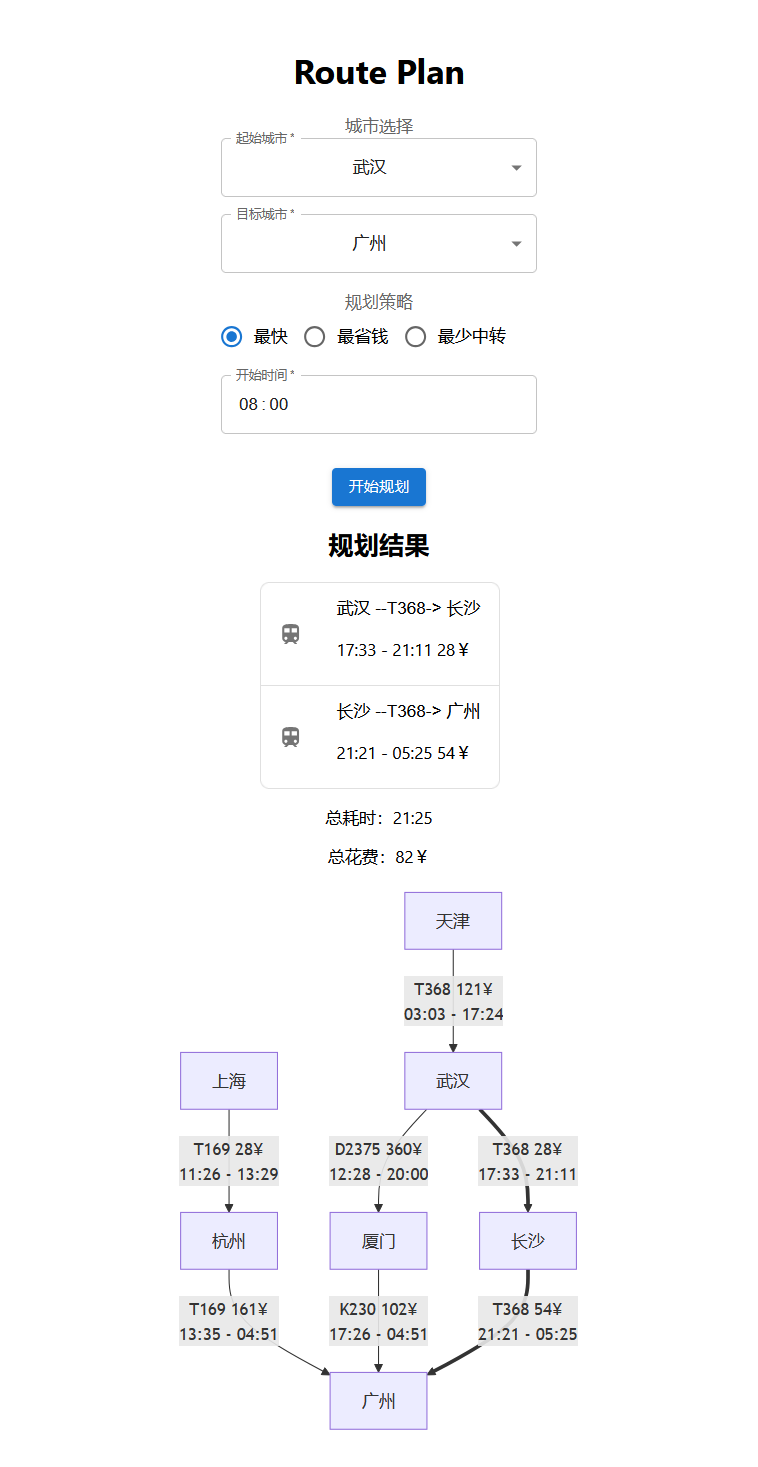
\includegraphics[width=0.7\linewidth]{img/screenshot008}
        \caption{最快路径规划结果-exp1-1}
        \label{fig:screenshot008}
    \end{figure}

    \paragraph{exp2-1}
    如果此时添加一条从厦门到广州的列车,但是恰好在20:00之后发车,可以看到如图\ref{fig:screenshot009}所示,现在选择途径厦门。

    这是因为虽然途径厦门的全程时间要比途径长沙的全程时间长,但是因为设置为08:00出发,考虑到了等待第一班车的时间,所以还是选择途径厦门。
    \begin{figure}
        \centering
        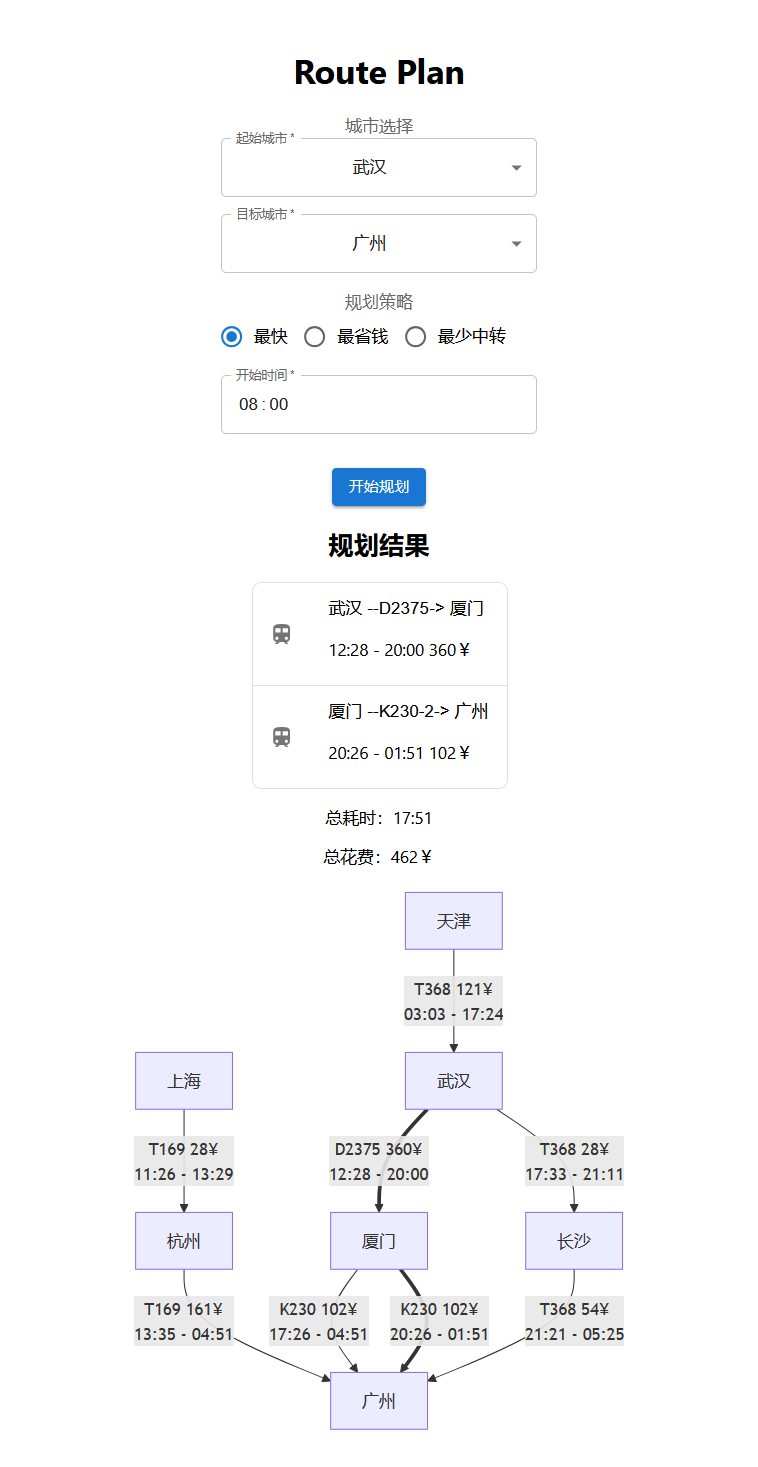
\includegraphics[width=0.7\linewidth]{img/screenshot009}
        \caption{最快路径规划结果-exp2-1}
        \label{fig:screenshot009}
    \end{figure}

    \paragraph{exp2-2}
    此时,我们再把开始时间调到 14:00,可以看到如图\ref{fig:screenshot010}所示,此时又选择途径长沙,而不是选择途径厦门。

    这是因为14:00出发时,已经赶不上当日途径厦门的列车,所以会选择途径长沙。

    \begin{figure}
        \centering
        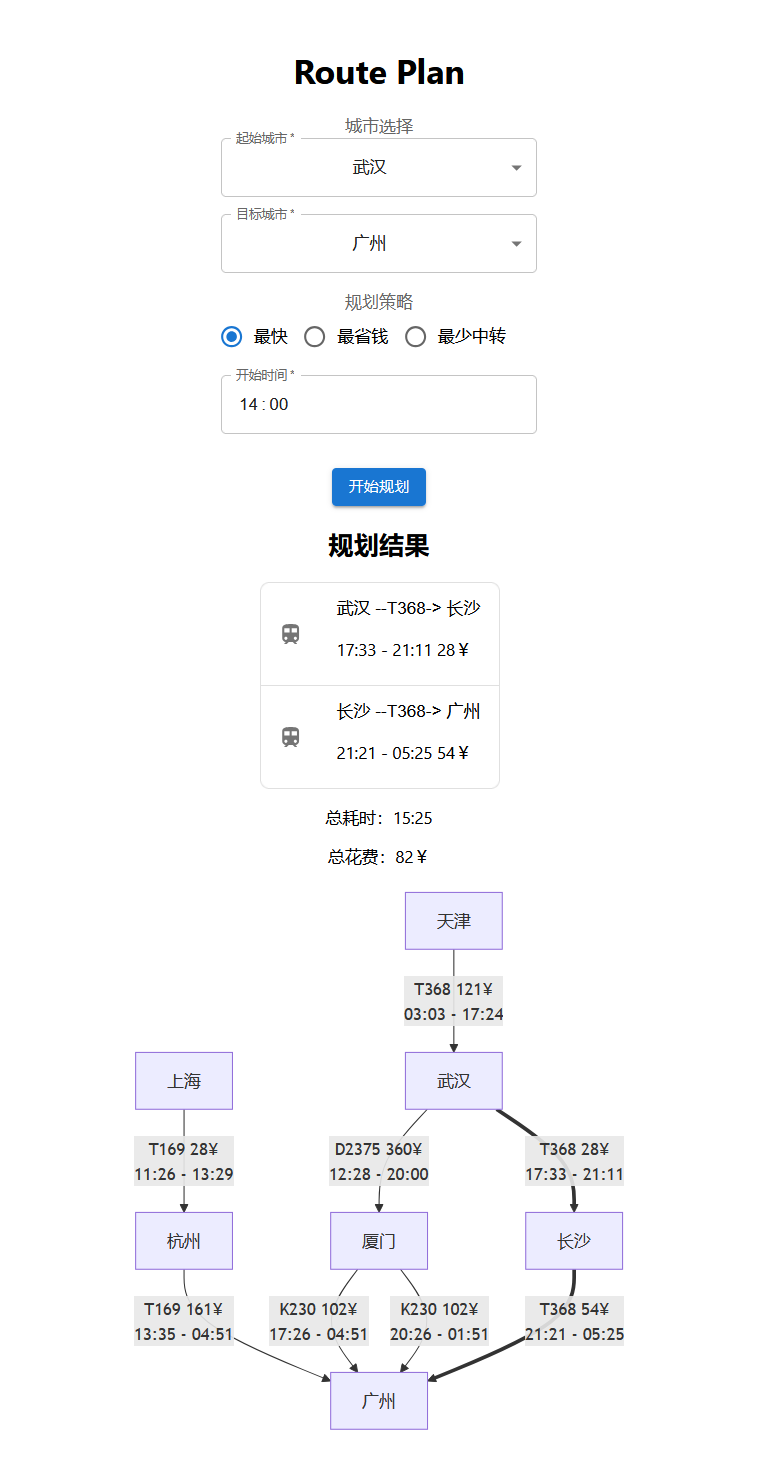
\includegraphics[width=0.7\linewidth]{img/screenshot010}
        \caption{最快路径规划结果-exp2-2}
        \label{fig:screenshot010}
    \end{figure}


    \section{项目亮点}
    \begin{itemize}
        \item 基于图数据结构的路径规划系统:通过使用图数据结构,可以轻松地实现路径规划,包括最省钱、最少中转和最快到达三种策略。
        \item 高效的算法设计:使用优化后的 Dijkstra 算法,避免了传统的遍历算法的 $O(n!)$的时间复杂度
        \item 直观的用户交互:可以轻松地添加、删除和修改城市和交通路线的数据,实现数据的动态更新。
        \item 可视化展示功能:可以轻松地展示规划结果,包括时间、成本、中转次数等指标。
        \item 高效的数据处理能力:可以处理大规模数据,包括15个城市、4130条交通路线的数据集。
    \end{itemize}

    \section{总结}

    \subsection{项目成果}
    本项目成功实现了一个全国交通咨询模拟系统,主要取得了以下成果:

    \begin{itemize}
        \item 实现了基于图数据结构的路径规划系统,支持最快到达、最省钱和最少中转三种规划策略。
        \item 开发了完整的前后端分离架构,前端提供直观的用户界面,后端提供高效的算法实现。
        \item 成功处理了复杂的时间约束问题,包括等待时间、过夜等情况的合理计算。
        \item 支持大规模数据处理,目前可处理15个城市、4130条交通路线的数据集。
        \item 提供了完善的数据管理功能,包括城市和交通路线的增删改查。
        \item 实现了路线的可视化展示功能,直观展示规划结果。
    \end{itemize}
    
    \subsection{项目不足}
    尽管项目已经基本实现了预期功能,但仍存在以下不足:

    \begin{itemize}
        \item 数据存储方式较为简单,仅使用JSON文件存储,缺乏数据库支持。
        \item 路线可视化功能在大规模数据下性能欠佳,仅适用于小规模数据展示。
        \item 算法优化空间仍然较大,在处理大规模数据时性能可能受到影响。
        \item 系统安全性和容错性有待加强,缺乏完善的异常处理机制。
    \end{itemize}
    
    \subsection{未来改进方向}
    针对项目存在的不足,提出以下改进建议:

    \begin{itemize}
        \item 引入数据库系统,提升数据存储和查询效率。
        \item 优化路线可视化算法,提高大规模数据下的展示性能。
        \item 引入更多启发式算法,提升路径规划效率。
        \item 考虑引入实时数据,支持动态调整和实时更新。
        \item 增强系统的错误处理和日志记录功能。
        \item 优化系统架构,提高系统的可扩展性和维护性。
    \end{itemize}

    \appendix


    \section{附录}

    \subsection{项目仓库}
    \href{https://github.com/suyiiyii/DSExpDesign.git}{https://github.com/suyiiyii/DSExpDesign.git} \label{项目仓库}

    \subsection{城市数据}
    \href{https://github.com/suyiiyii/DSExpDesign/blob/main/data/city.json}{https://github.com/suyiiyii/DSExpDesign/blob/main/data/city.json} \label{city_data}

    \subsection{交通工具数据}
    \href{https://github.com/suyiiyii/DSExpDesign/blob/main/data/transport.json}{https://github.com/suyiiyii/DSExpDesign/blob/main/data/transport.json} \label{transport_data}

\end{document}